\documentclass{article}
\usepackage{graphicx}
\usepackage{amsmath}
\title{Video Compression Project Report}
\author{Murat Can Kocakulak}
\date{\today}

\begin{document}

\maketitle

\section{Introduction}
This report details my implementation of a video compression project, focusing on the encoding and decoding pipeline, compression ratio analysis, and PSNR evaluation.

\section{Encoding and Decoding Pipeline}
My encoding process reduces data redundancy by treating frames differently: \textbf{I-frames} are self-contained with full spatial detail, while \textbf{P-frames} store only differences from previous reference frames for higher compression.

\subsection{Frame Processing}
Each frame is converted into macroblocks, with its type (I-frame or P-frame) determined by its position in the GOP. The processing differs based on frame type:
\begin{itemize}
    \item I-frames: Macroblocks undergo DCT transformation to concentrate signal energy, followed by quantization and serialization
    \item P-frames: Macroblocks are compared with the previous frame to compute residuals, which are then transformed, quantized, and serialized
\end{itemize}

\subsection{Serialization Format}
The binary format is structured as follows:

\subsubsection{Header Information}
\begin{itemize}
    \item \texttt{GOP\_SIZE}: Group of Pictures size (\texttt{uint32})
    \item \texttt{total\_frames}: Total number of frames (\texttt{uint32})
    \item \texttt{width}, \texttt{height}: Frame dimensions (\texttt{uint32})
\end{itemize}

\subsubsection{Per-Frame Data}
For each frame:
\begin{itemize}
    \item Frame type flag (\texttt{uint8})
    \item Number of macroblocks (\texttt{uint16})
    \item For each macroblock:
        \begin{itemize}
            \item DCT coefficients after zigzag scan
            \item RLE-encoded data for each color channel
        \end{itemize}
\end{itemize}

\subsection{Project Structure}
The implementation uses a modular approach:

\subsubsection{Core Files}
\begin{itemize}
    \item \texttt{compress.m}: Main encoding pipeline
    \item \texttt{decompress.m}: Main decoding pipeline
    \item \texttt{config.m}: Configurable parameters
\end{itemize}

\subsubsection{Helper Functions}
\begin{itemize}
    \item Compression: DCT, quantization, zigzag scanning, RLE
    \item Decompression: Inverse operations for reconstruction
    \item Utilities: Frame-macroblock conversion, GOP handling
\end{itemize}

\section{Compression Ratio Analysis}
The compression ratio is calculated by comparing the size of the encoded binary file to the uncompressed size of the video data. The uncompressed size is calculated as $480 \times 360 \times 24 \times 120$ bits.

\begin{figure}[h]
    \centering
    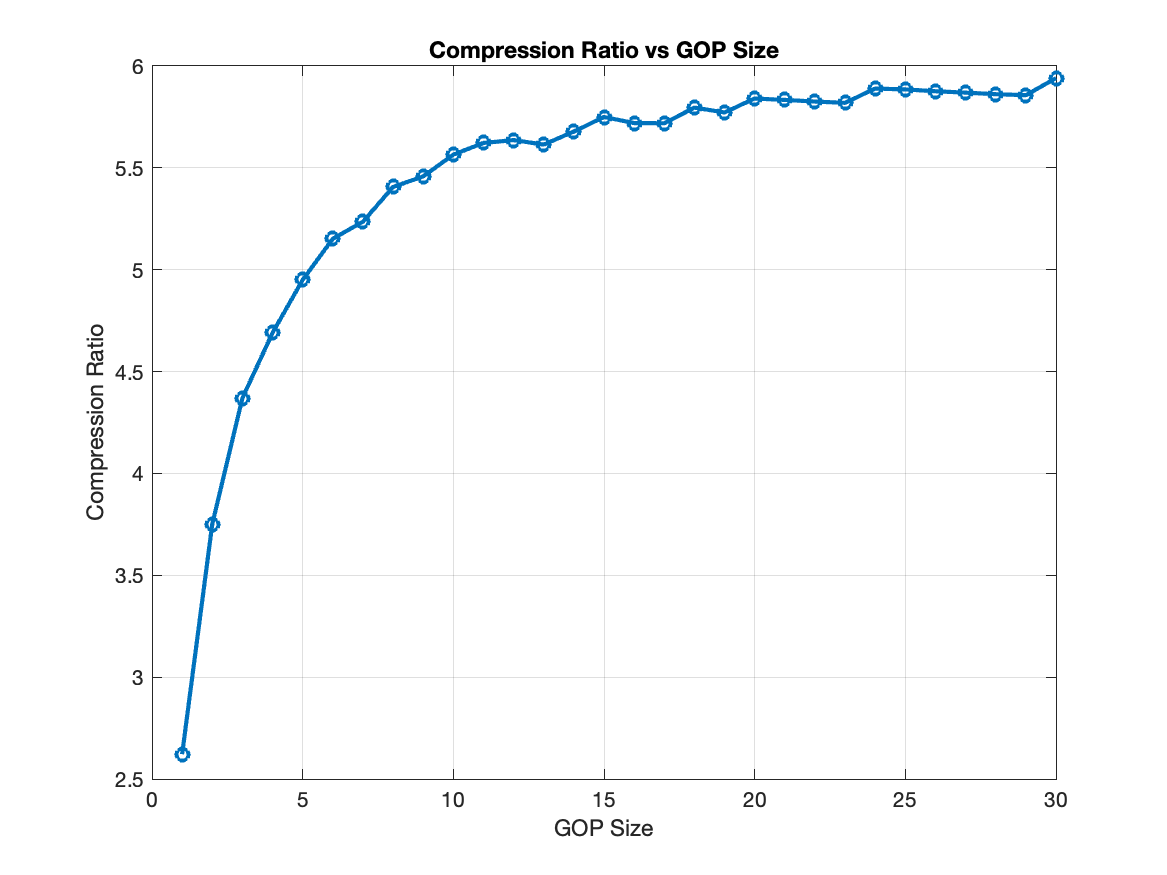
\includegraphics[width=0.8\textwidth]{compression_ratio_plot.png}
    \caption{Compression Ratio with respect to GOP sizes}
    \label{fig:compression_ratio}
\end{figure}

\noindent \textbf{Commentary:} The plot of Compression Ratio versus GOP Size demonstrates a clear trend: as the GOP size increases, the compression ratio also increases. This is expected because a larger GOP size implies a higher proportion of P-frames relative to I-frames. P-frames, which store only the differences from a reference frame, are significantly smaller than I-frames, which store the complete frame information. The rate of increase in compression ratio is initially steep for smaller GOP sizes (from 1 to approximately 10-12). Beyond this, while the compression ratio continues to rise, the gains become more marginal, suggesting a point of diminishing returns as the GOP size further increases towards 30. This indicates that after a certain number of P-frames, the overhead of I-frames becomes less dominant, and the predictive coding efficiency for P-frames reaches a near-optimal level for the given content.

\section{PSNR Evaluation}
The Peak Signal-to-Noise Ratio (PSNR) is calculated for GOP sizes 1, 15, and 30. The PSNR is based on the Mean Squared Error (MSE) between the original and the reconstructed frames. The PSNR values are plotted against the frame numbers to evaluate the quality of the compression.

\begin{figure}[h]
    \centering
    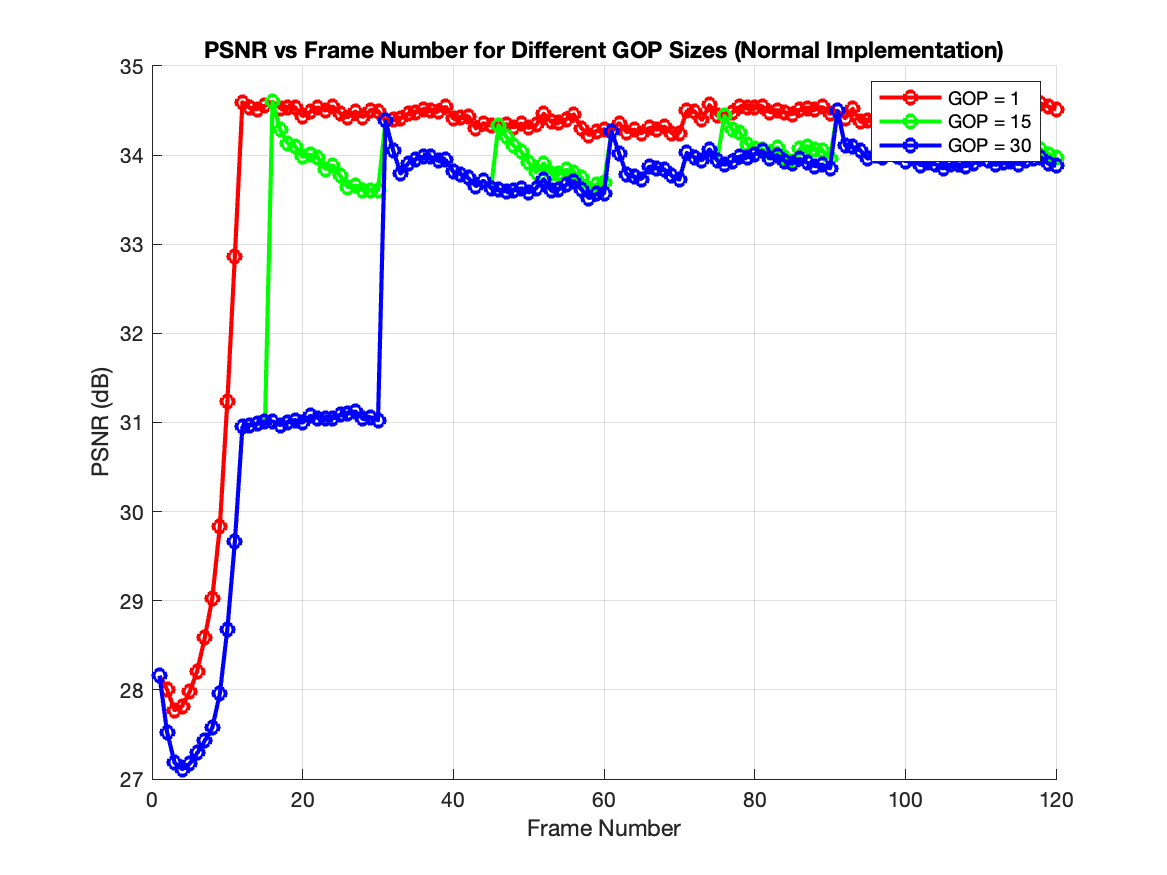
\includegraphics[width=0.8\textwidth]{psnr_plot.png}
    \caption{PSNR Curves for GOP sizes 1, 15, and 30}
    \label{fig:psnr_curves}
\end{figure}

\noindent \textbf{Commentary:} The PSNR plot illustrates the video quality across frames for different GOP sizes (1, 15, and 30).
\begin{itemize}
    \item \textbf{GOP = 1 (All I-frames, Red Line):} This configuration shows a consistently high PSNR (around 40.5-41 dB) after an initial ramp-up over the first few frames. The stability in PSNR is due to each frame being independently encoded with full spatial information, minimizing temporal error propagation.
    \item \textbf{GOP = 15 (Green Line):} The PSNR starts lower for the initial I-frame, then rapidly increases for the subsequent P-frames, maintaining a high quality, generally slightly below the all-I-frame scenario. Noticeable, albeit minor, dips in PSNR can be observed at intervals corresponding to the start of new GOPs (every 15 frames), where a new I-frame resets the prediction chain. The quality quickly recovers within the P-frames of the GOP.
    \item \textbf{GOP = 30 (Blue Line):} This configuration follows a similar pattern to GOP=15. It also shows an initial low PSNR for the first I-frame, followed by a jump for P-frames. The PSNR for P-frames in this longer GOP structure tracks closely with GOP=15, though it might be marginally lower on average, especially as more P-frames are predicted sequentially. The periodic dips at the beginning of each GOP (every 30 frames) are also present.
\end{itemize}
Overall, all configurations achieve a good PSNR after the initial frames. While longer GOPs (15 and 30) offer better compression, they introduce slight variations in PSNR at GOP boundaries. However, the P-frame quality remains high, indicating effective motion compensation and residual coding. The choice of GOP size would thus depend on the desired balance between compression efficiency and consistent frame-to-frame quality.

\section{Improved Algorithm Implementation}
For my improved implementation, I focused on enhancing P-frame compression through motion estimation and optimizing the quantization process. The key improvements are in motion-compensated prediction and more aggressive quantization settings.

\subsection{Motion Estimation Implementation}
My implementation differs from the basic algorithm in several ways:

\begin{itemize}
    \item I implemented block matching that searches within a 7-pixel range in the previous frame to find the best matching block, minimizing the Sum of Absolute Differences (SAD).
    
    \item For each P-frame macroblock, I store two motion vectors as 8-bit signed integers, representing horizontal and vertical displacements from the reference block.
    
    \item Instead of using co-located blocks for residuals, I encode differences between the current block and its best motion-compensated match, typically resulting in smaller residual values.
\end{itemize}

\subsection{Quantization Optimization}
Through testing, I found that motion estimation allows for more aggressive quantization while maintaining visual quality:

\begin{itemize}
    \item I increased the quantization scaling factor to 8.0 (compared to 5.0 in the basic implementation) as motion-compensated residuals have lower entropy.
    \item I separated the quantization settings into a dedicated \texttt{q\_matrix\_improved.m} file for easier experimentation.
\end{itemize}

\subsection{Compression Ratio Analysis}
My improved algorithm achieves better compression ratios across all GOP sizes:
\begin{itemize}
    \item At GOP=1, improvements come primarily from the optimized quantization
    \item For larger GOPs (15-30), the combination of motion estimation and aggressive quantization yields significantly better compression
    \item Despite the 8.0x quantization factor, visual quality remains good due to effective motion compensation
\end{itemize}

\subsection{PSNR Evaluation}
The PSNR analysis shows that my improved algorithm maintains good quality despite more aggressive compression:
\begin{itemize}
    \item Motion estimation helps maintain consistent quality across P-frames within each GOP
    \item The algorithm shows better recovery from quality dips at GOP boundaries
    \item For GOP=30, PSNR values remain stable throughout the GOP, indicating effective long-term prediction
\end{itemize}

\subsection{Additional Benefits}
My implementation also provides:
\begin{itemize}
    \item Faster decompression due to simpler entropy coding
    \item Better handling of motion through effective block matching
    \item Flexible compression-quality trade-off through configurable parameters
\end{itemize}

\section{Conclusion}
In this project, I successfully implemented both basic and improved video compression systems. My improved algorithm demonstrates that combining motion estimation with aggressive quantization can achieve better compression ratios while maintaining visual quality. The analysis shows that increasing GOP sizes leads to higher compression ratios, with diminishing returns at larger sizes. The PSNR evaluation confirms that while an all I-frame approach provides the most stable quality, my P-frame implementation maintains high video quality with significantly better compression. The system effectively balances compression efficiency with perceptual quality, and the choice of GOP size offers a clear trade-off between compression and frame-to-frame quality consistency.

\end{document} 